\chapter{Analyse des performances et parallélisation}
\section{L'information de base de l'ordinateur}
Nous pouvons utiliser la commande \texttt{wmic cpu get} pour obtenir le nombre de cœurs physiques et les tailles des caches, ou bien consulter directement le Gestionnaire des tâches dans l'onglet Performance, où l'on peut voir les informations matérielles de l'appareil, y compris le nombre de cœurs physiques, le nombre de processeurs logiques et la taille des caches L1/L2/L3.

\begin{table}[h]
\centering
\begin{tabular}{|c|c|}
\hline
\multicolumn{2}{|c|}{Information de base de l'ordinateur} \\  
\hline
Nombre de cœurs physiques  & 12 \\  
\hline
Cache L1 & 1.1 MB \\  
\hline
Cache L2 & 9.0 MB \\  
\hline
Cache L3 & 18.0 MB\\  
\hline
\end{tabular}
\caption{Information de base de l'ordinateur}
\label{tab:instructions}
\end{table}

\section{Le temps moyen de l'exécution}
En effectuant quelques modifications du programme \texttt{Model::update()} dans le fichier \texttt{model.cpp}, nous pouvons obtenir le résultat suivant, où le temps d'exécution moyen par time step est d'environ \textbf{782$\mu$s}.
\begin{figure}[h]
    \centering
    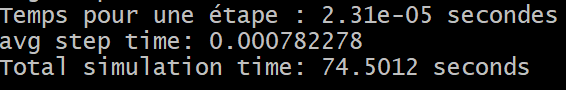
\includegraphics[width=1.1\linewidth]{fig1.png}
    \caption{Résultat séquentiel}
    \label{fig:enter-label}
\end{figure}
Ici, le temps total de la simulation du incendie avec n=100 de cases par direction pour la discrétisation et la position du foyer initial s = (50,50).
\section{Parallélisation avec OpenMP}
On inclut \texttt{<omp.h>} et implémente la parallélisation dans \texttt{Model::update()}.
\begin{table}[h]
    \centering
    \resizebox{0.8\textwidth}{!}{
        \begin{tabular}{|c|c|c|c|c|} 
            \hline 
              & n thread = 1 & n thread = 2 & n thread = 4 & n thread = 8 \\
            \hline
            Temps moyen de chaque avancement (ms) & 121.9 & 85 & 37.8 & 29.7 \\
            Temps total (s) & 159.5 & 134.2 & 104.6 & 88.9 \\
            speedup de temps moyen & 1.00 & 1.43 & 3.22 & 4.10 \\
            speedup de temps total & 1.00 & 1.19 & 1.52 & 1.79 \\
            \hline
            \end{tabular}
    }
    \caption{Résultat de la parallélisation avec OpenMP}
    \label{tab:mytable}
\end{table}
\begin{figure}[h]
    \centering
    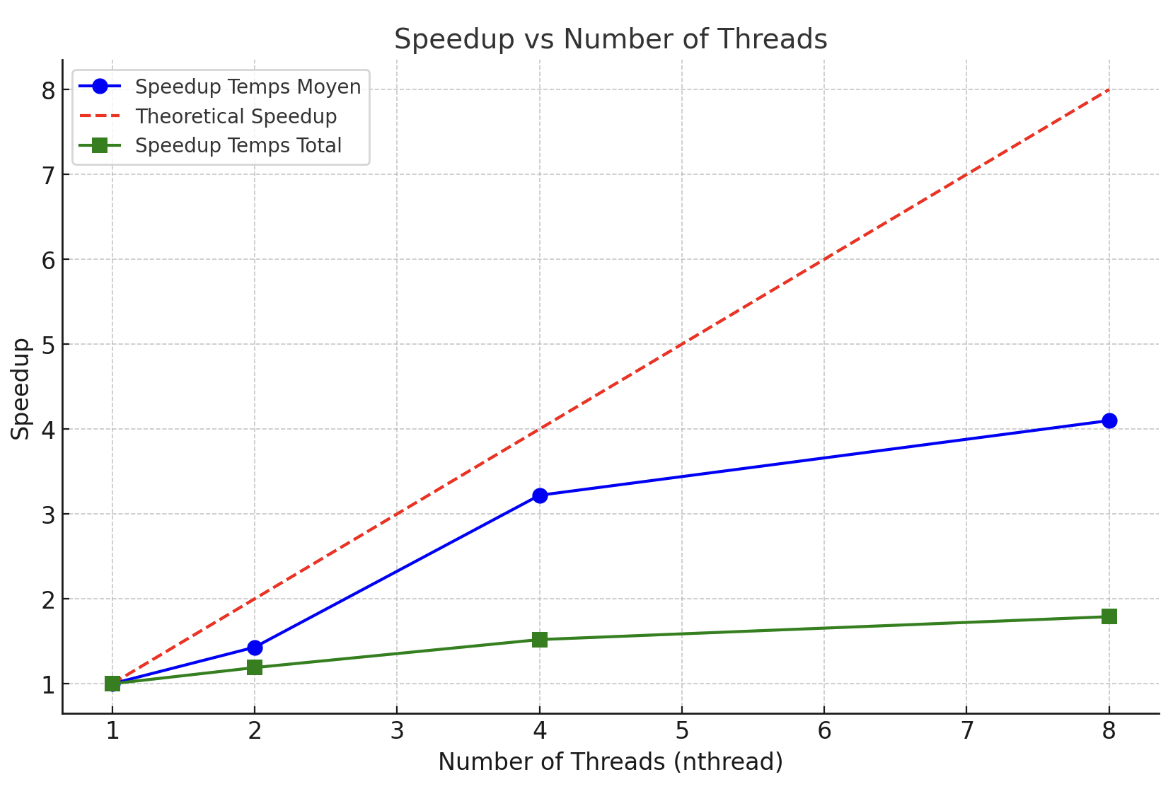
\includegraphics[width=0.9\linewidth, height=0.5\textwidth]{speedup_openmp.png}
    \caption{Speedup de l'avancement}
    \label{fig:enter-label}
\end{figure}
\par
On peut voir que la parallélisation avec OpenMP améliore grandement les performances du programme. Mais il faut noter que le speedup n'est pas toujours linéaire avec le nombre de threads, l’amélioration de la parallélisation n’est pas significative par rapport au code original exécuté séquentiellement, ce qui peut être dû aux coûts de communication et de synchronisation entre les processus.